\section{Historic perspective}

\begin{frame}[t]{Computer technology}

\mode<presentation>{\vspace{-1em}}
\begin{columns}[T]

\column{.45\textwidth}
\textgood{ASCI Red Computer}: \textemph{1.3 TFLOPS}\\
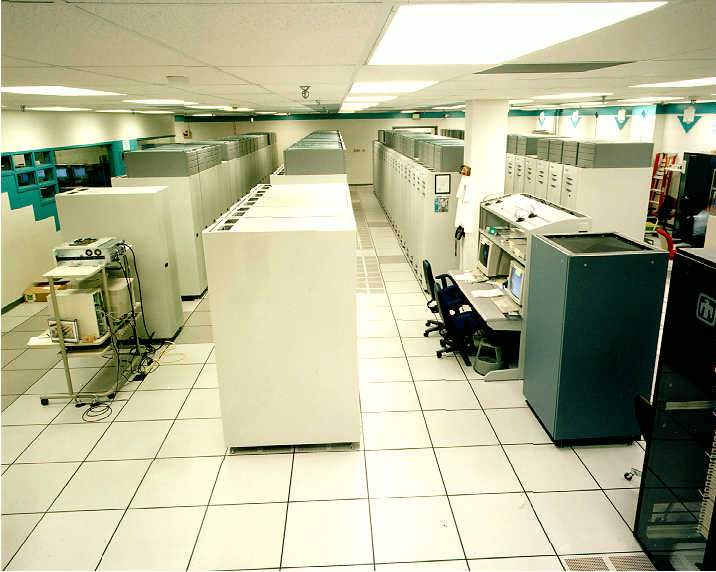
\includegraphics[height=.6\textheight]{images/asci-red.jpg}\\
\begin{tiny}
By Sandia National Laboratories, Public Domain\\
\url{https://commons.wikimedia.org/w/index.php?curid=28171282}\\
\end{tiny}

\textmark{1997}\\

\pause

\column{.55\textwidth}
\textgood{Samsung S22}: \textemph{1.2 -- 2.2 TFLOPS}\\
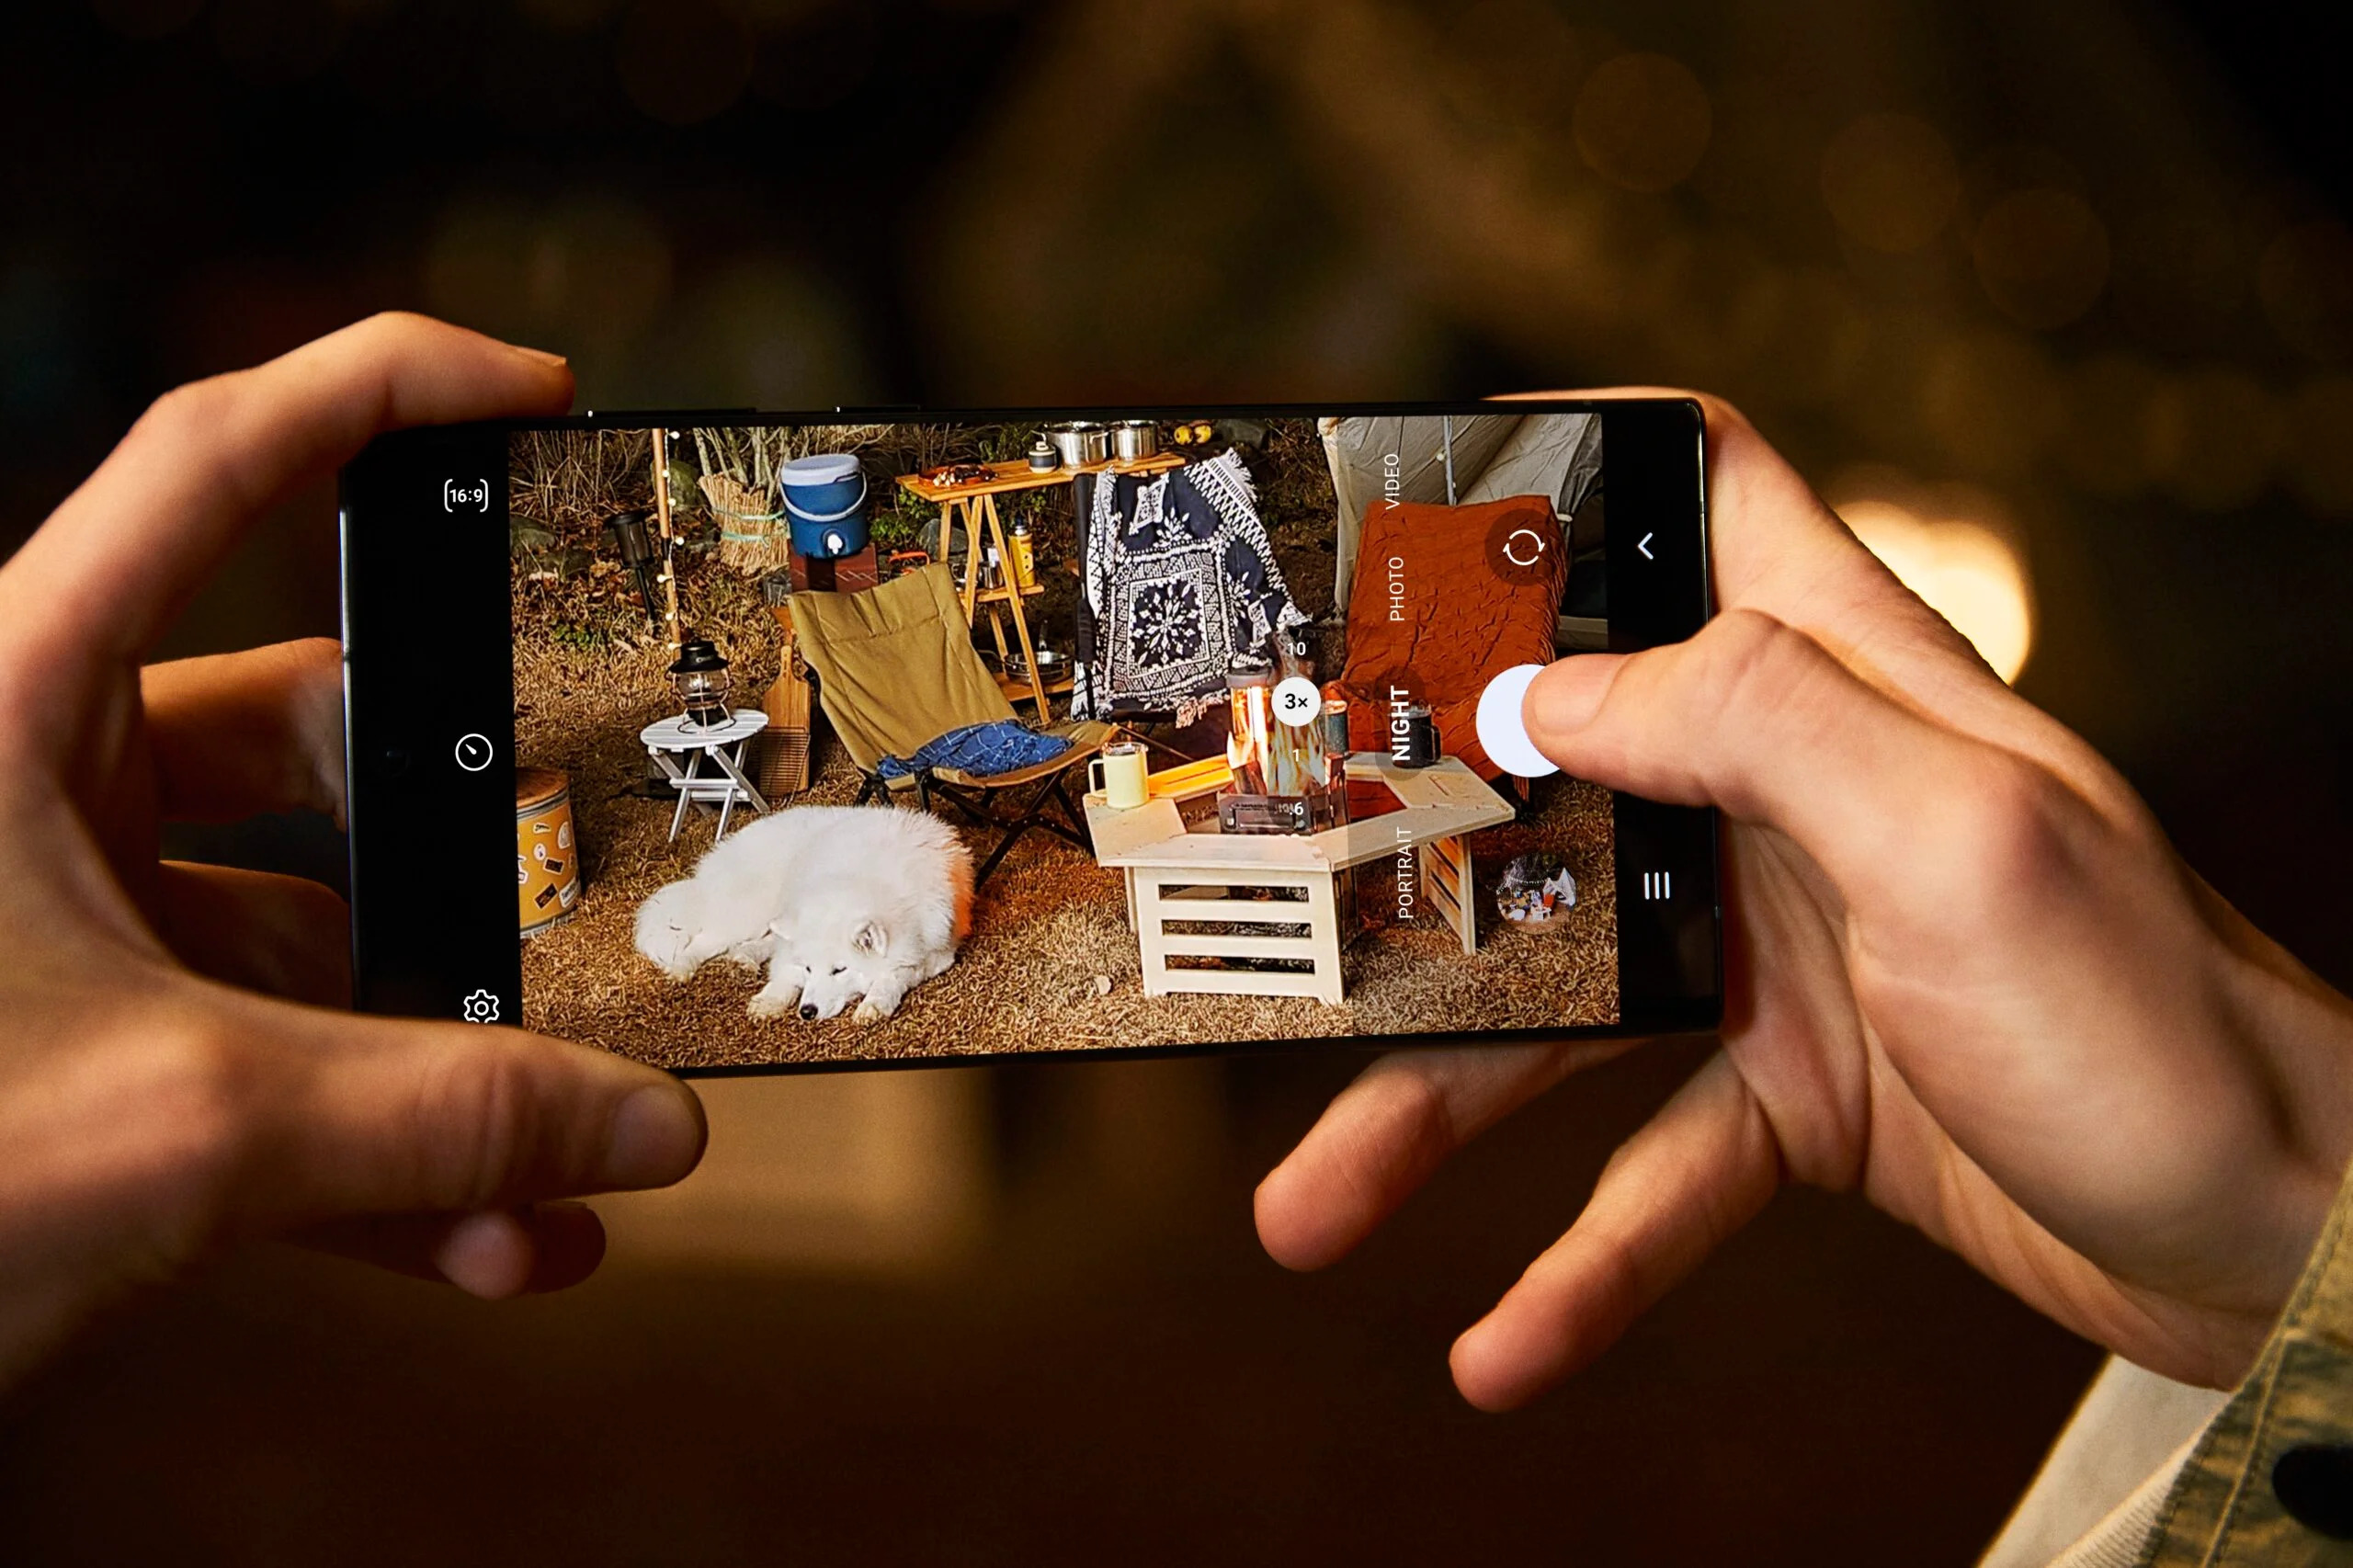
\includegraphics[height=.6\textheight]{images/samsung-s22.jpg}\\
\begin{tiny}
By Trusted Reviews, Creative Commons BY-NC-ND 4.0\\
{\begin{spacing}{1.0}
\url{https://www.trustedreviews.com/versus/samsung-galaxy-s22-ultra-vs-samsung-galaxy-s22-plus-vs-samsung-galaxy-s22-4207904}
\end{spacing}}
\end{tiny}

\textmark{2022}\\

\end{columns}

\end{frame}


\begin{frame}[t]{First revolution: Microprocessor}
\begin{itemize}
  \item The microprocessor revolution.
    \begin{itemize}
      \item Generated from a single change.
      \item Enough transistors (25,000) in a single chip for a 16-bit processor.
      \item \bulletgood{Advantages}:
        \begin{itemize}
          \item \bulletmark{Faster}: Less accesses out of the chip.
          \item \bulletmark{Cheaper}: All in one chip.
        \end{itemize}
    \end{itemize}
  \item New market segments generated by the innovation.
    \begin{itemize}
      \item Desktop computers, CD/DVD, laptops, video-game consoles, set-top-boxes,
            digital cameras, MP3, GPS, \ldots
    \end{itemize}
  \item Impact on existing markets.
    \begin{itemize}
      \item Supercomputers, mainframes, \ldots
    \end{itemize}
\end{itemize}
\end{frame}

\begin{frame}[t]{First microprocessor}
\begin{columns}[T]
  \begin{column}{.7\textwidth}
    \begin{itemize}
      \item Intel 4004 (1971).
        \begin{itemize}
          \item \bulletmark{Application domain}: Calculators.
          \item \bulletmark{Technology}: 10,000 nm.
          \mode<presentation>{\vfill}
          \item \bulletenum{Data}:
            \begin{itemize}
              \item 2300 transistors.
              \item 13 mm2
              \item 108 KHz
              \item 12 Volts
            \end{itemize}
          \mode<presentation>{\vfill}
          \item \bulletenum{Features}:
            \begin{itemize}
              \item 4-bits data.
              \item Data-path in one cycle.
            \end{itemize}
      \end{itemize}
    \end{itemize}
  \end{column}
  \begin{column}{.3\textwidth}
    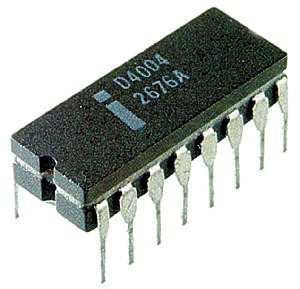
\includegraphics[width=.5\textwidth]{images/intel-4004.jpg}\\
    \begin{tiny}
      \emph{Intel 4004} photo by Rostislav Lisovy\\
    \end{tiny}
    \vspace{1em}
    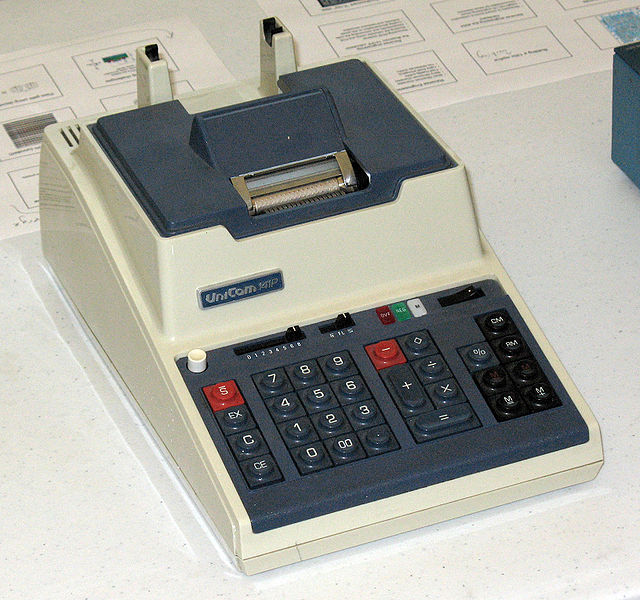
\includegraphics[width=.5\textwidth]{images/i4004-calculator.jpg}\\
    \begin{tiny}
      \emph{Unicom 141P Calculator 3} photo by Michael Holley.\\ 
    \end{tiny}
  \end{column}
\end{columns}
\end{frame}

\begin{frame}[t]{Effects of microprocessors}
\begin{itemize}
  \item \textmark{Mass production} of microprocessors
    \begin{itemize}
      \item Strong reduction in unit cost.
      \item Increasing fraction of computers based in microprocessors.
    \end{itemize}

  \mode<presentation>{\vfill\pause}
  \item Significant \textgood{changes} in computer marketplace:
    \begin{itemize}
	\item Nearly \textbad{eliminated} need for \textmark{assembly programming}.
      \item \textgood{Standardized} vendor independent \textmark{operating systems}.
        \begin{itemize}
          \item UNIX $\rightarrow$ Linux
        \end{itemize}
      \item \textgood{Lower costs} for newer architectures.
    \end{itemize}
\end{itemize}
\end{frame}

\begin{frame}[t]{Second revolution}
\begin{itemize}
  \item Extract implicit instruction-level parallelism (ILP).
    \begin{itemize}
      \item Hardware has resources that can be used in parallel.
    \end{itemize}
  \vfill
  \pause
  \item \bulletenum{Elements}:
    \begin{itemize}[<+->]
      \item \bulletmark{Pipelining}: Allowed increasing clock frequency.
      \item \bulletmark{Caches}: Needed to increase clock frequencies.
      \item \bulletmark{Floating point}: Integrated into the chip.
      \item Increasing pipeline \bulletmark{depth} and \bulletmark{speculative branching}.
      \item \bulletmark{Multiple issue}: superscalar architectures.
      \item \bulletmark{Dynamic scheduling}: Out-of-Order execution.
    \end{itemize}
\end{itemize}
\end{frame}

\begin{frame}[t,shrink=15]{Top single core processors}
\begin{columns}
  \begin{column}{.15\textwidth}
    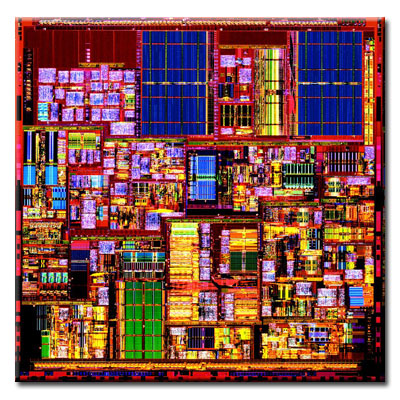
\includegraphics[width=\textwidth]{images/intel-p4-die.jpg}\\
    \begin{tiny}
      Die of Intel Pentium 4 (Northwood)\\ 
      Source: \url{http://gecko54000.free.fr}\\
    \end{tiny}
    \vspace{0.75em}
    \begin{center}
      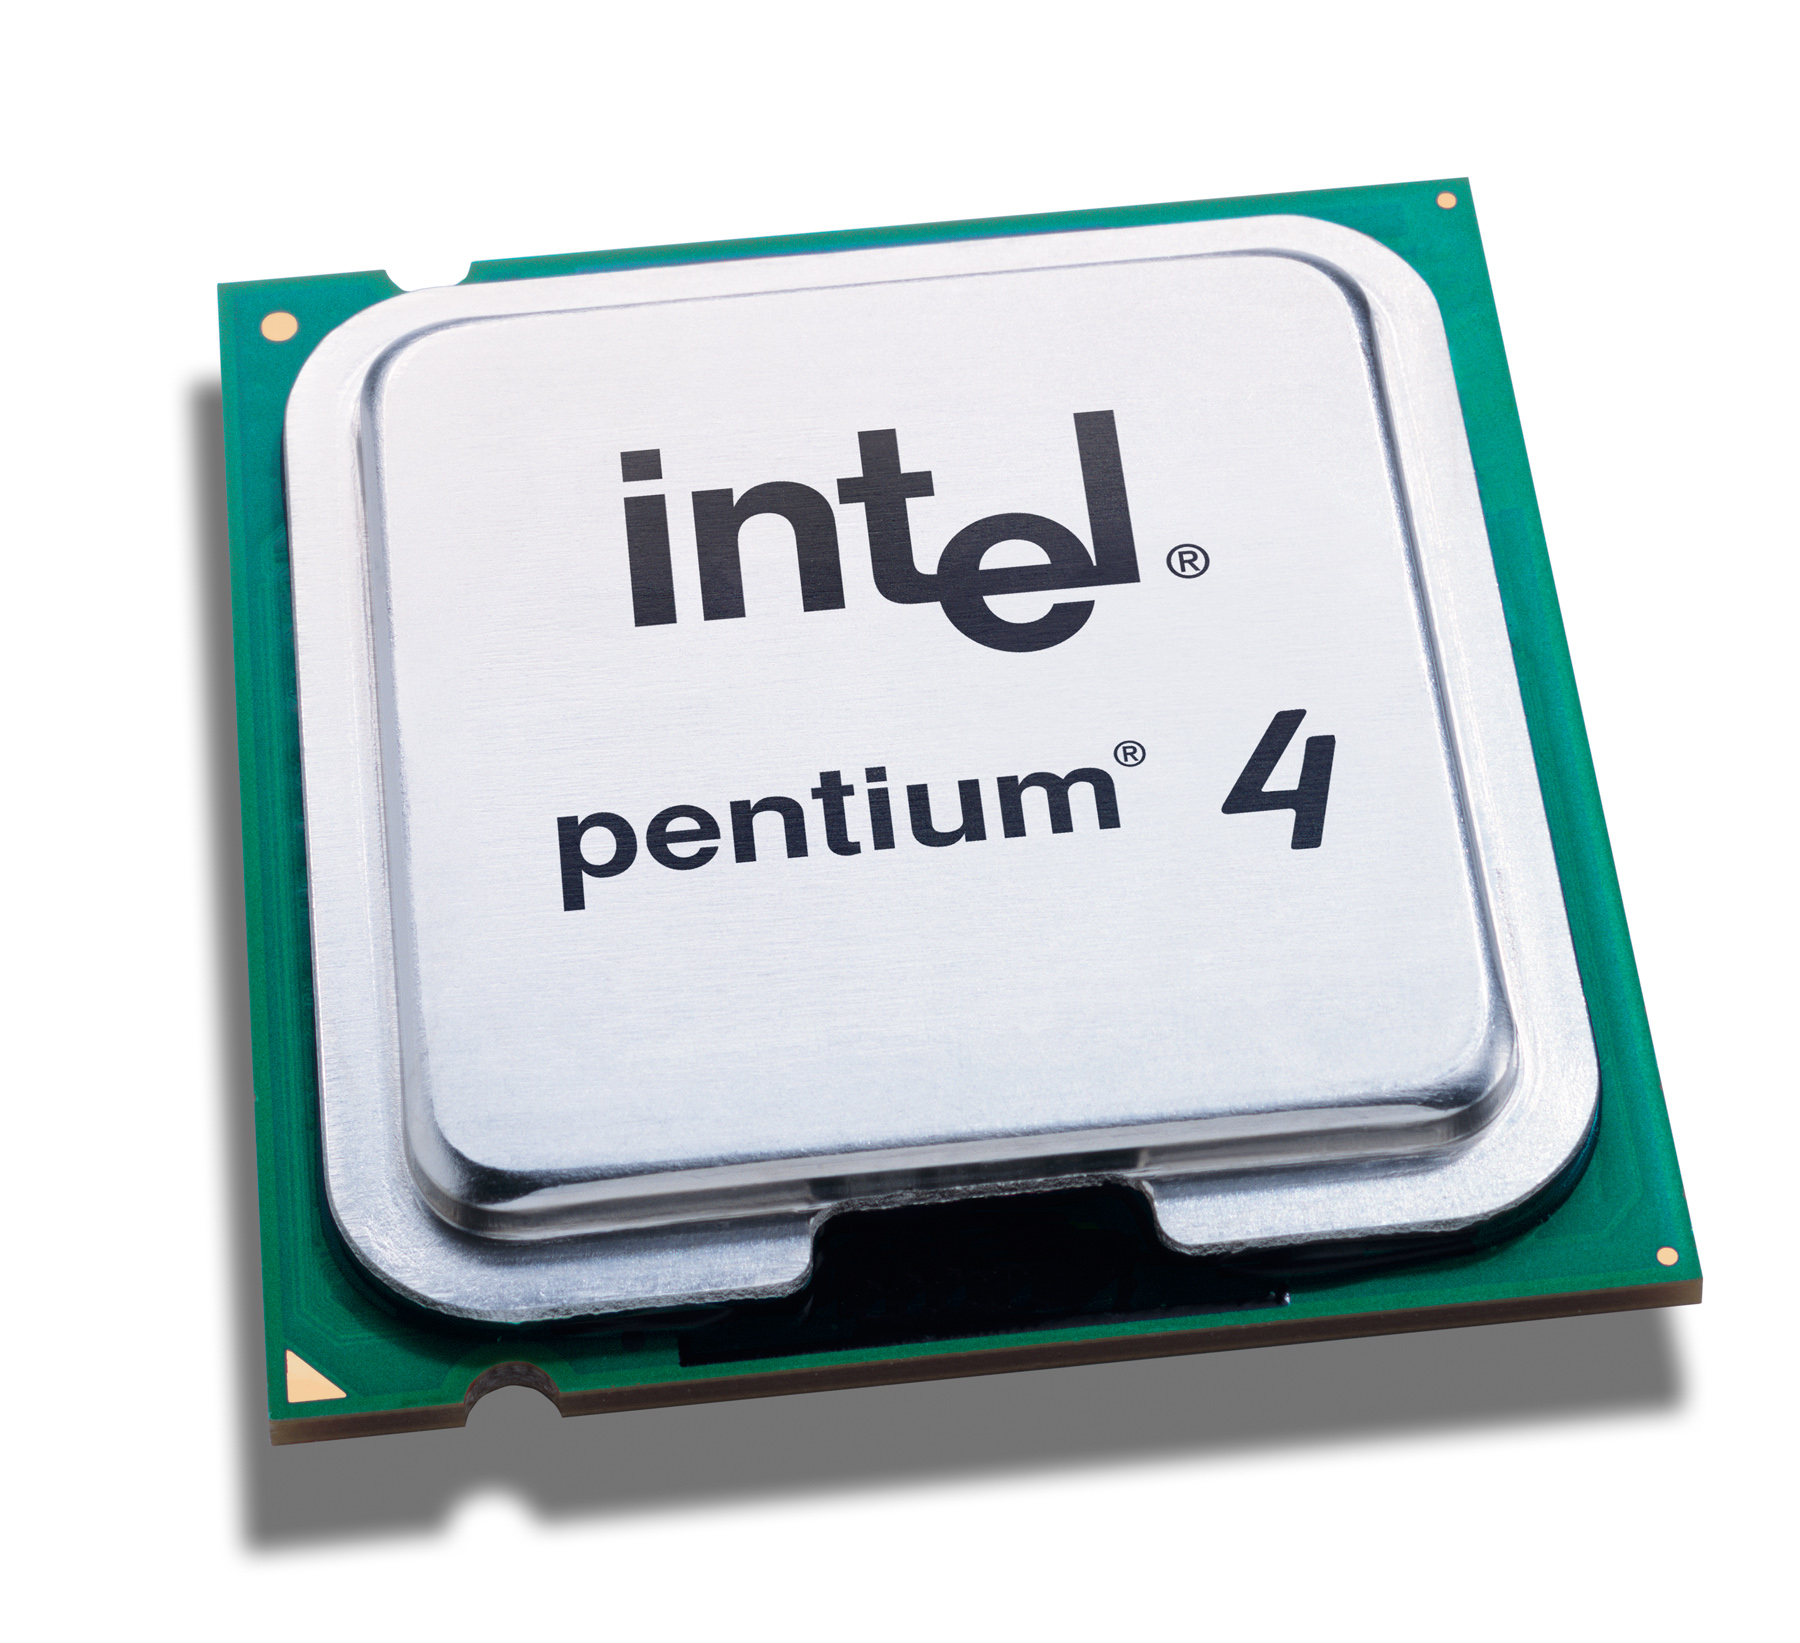
\includegraphics[width=.9\textwidth]{images/intel-p4.jpg}\\
    \end{center}
  \end{column}
  \begin{column}{.7\textwidth}
    \begin{itemize}
      \item Intel Pentium 4 (2003).
        \begin{itemize}
          \item \bulletmark{Application domain}: Desktop / Servers.
          \item \bulletmark{Technology}: 90 nm (1/100x).
        \end{itemize}
      \item \bulletenum{Data}:
        \begin{itemize}
          \item 55M transistors (20,000x).
          \item 101 mm$^2$ (10x).
          \item 3.4 GHz (10,000x).
          \item 1.2 Volts (1/10x).
        \end{itemize}
      \item \bulletenum{Features}:
        \begin{itemize}
          \item 32/64-bit data (16x).
          \item Data path with 22 pipeline stages (later 31).
          \item 3-4 instructions per cycle (superscalar).
          \item Two level cache on chip.
          \item Data parallel instructions (SIMD).
          \item Hyper-threading.
        \end{itemize}
    \end{itemize}
  \end{column}
\end{columns}
\end{frame}

\begin{frame}[t]{Third revolution}
\begin{itemize}
  \item Explicitly support thread-level and data-level parallelism.
    \begin{itemize}
      \item Hardware offers parallel resources and software specifies its use.
      \item Parallelism no longer hidden by hardware.
      \item \bulletmark{Rationale}: Diminishing returns from ILP.
    \end{itemize}
  \mode<presentation>{\vfill\pause}
  \item \bulletenum{Elements}:
    \begin{itemize}
      \item \bulletmark{Vector instructions}: Intel SSE, AVX, AVX-2 \ldots.
      \item General support for \bulletmark{multi-threaded} applications.
    \end{itemize}
\end{itemize}
\end{frame}

\begin{frame}[t,shrink=20]{Multi-core processors}
\begin{columns}[T]
  \begin{column}{.65\textwidth}
    \begin{itemize}
      \item Intel Core i7 (2009).
        \begin{itemize}
          \item \bulletmark{Application}: Desktop / Server.
          \item \bulletmark{Technology}: 45 nm (1/2x).
        \end{itemize}
      \item \bulletenum{Data}:
        \begin{itemize}
          \item 774M transistors (12x).
          \item 296 mm$^2$ (3x).
          \item 3.2 GHz -- 3.6 GHz ($\approx$1x).
          \item 0.7 -- 1.4 Volts ($\approx$1x).
        \end{itemize}
      \item \bulletenum{Features}:
        \begin{itemize}
          \item 128-bit data (2x).
          \item Datapath with 14-stage pipeline (0.5x).
          \item 4 instructions per cycle ($\approx$1x).
          \item Three level cache on chip.
          \item Data parallel instructions (SIMD).
          \item Hyper-threading.
          \item 4 cores (4x).
        \end{itemize} 
    \end{itemize}
  \end{column}
  \begin{column}{.35\textwidth}
    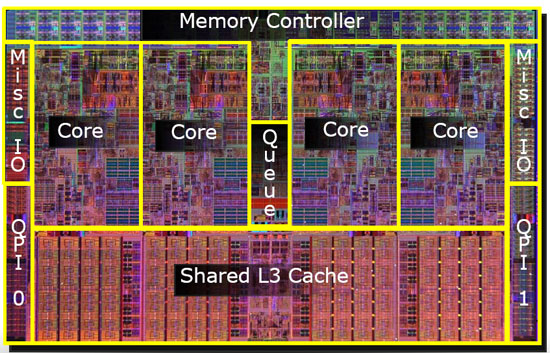
\includegraphics[width=.9\textwidth]{images/intel-core-i7-die.jpg}\\
    \begin{tiny}
      Die of Intel Core i7 (Nehalem)\\
      Source: \url{www.legitreviews.com}\\
    \end{tiny}
    \vspace{0.75em}
    \begin{center}
    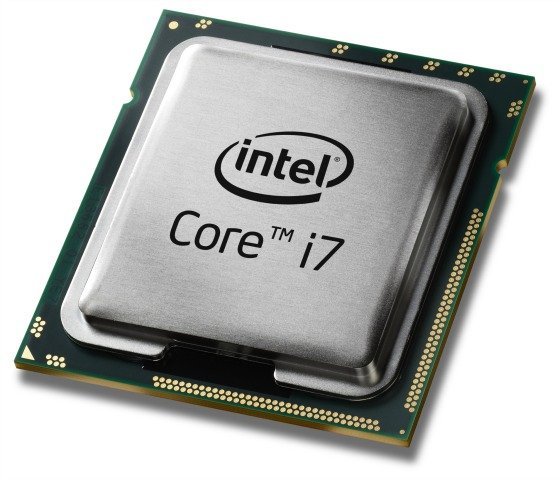
\includegraphics[width=.45\textwidth]{images/intel-core-i7.jpg}\\
    \end{center}
  \end{column}
\end{columns}
\end{frame}

\begin{frame}[t]{Architecture trends}
\begin{itemize}
  \item Instruction-Level Parallelism.
    \begin{itemize}
      \item Parallel execution of instructions.
      \item Impossible to improve Instruction-Level parallelism (since 2003-2005).
      \item Hardware and compiler conspiration to hide details to programmer.
        \begin{itemize}
          \item Programmer with \alert{very simplified} view of hardware.
        \end{itemize}
    \end{itemize}
  \mode<presentation>{\pause\vfill}
  \item New models to improve performance.
    \begin{itemize}
       \item \bulletmark{Data-Level} Parallelism (DLP).
       \item \bulletmark{Thread-Level} Parallelism (TLP).
       \item \bulletmark{Request-Level} Parallelism (RLP).
    \end{itemize}
  \mode<presentation>{\pause\vfill}
  \item \alert{IMPORTANT}: All of them require to re-structure applications to
        take advantage of promised performance increase.
\end{itemize}
\end{frame}

